% !TeX program = pdflatex
% Gallery starter; see TEMPLATE-README.txt for attribution and licenses.
\documentclass[20pt]{extarticle}
\usepackage[paperwidth=46cm,paperheight=65cm,margin=25mm]{geometry}
\usepackage[T1]{fontenc}\usepackage{lmodern,microtype,multicol,xcolor,graphicx,booktabs,tikz}
\definecolor{ink}{HTML}{173F4F}\definecolor{accent}{HTML}{D4783D}
\usepackage{titlesec}\titleformat{\section}{\Large\sffamily\bfseries\color{accent}}{}{0pt}{}
\setlength{\parindent}{0pt}\setlength{\parskip}{12pt}\setlength{\columnsep}{22mm}\pagestyle{empty}
\begin{document}
{\sffamily\color{accent}RESEARCH SHOWCASE / 2026\par}
\vspace{12mm}{\sffamily\bfseries\color{ink}\fontsize{57}{64}\selectfont Making research\\easier to reproduce\par}
\vspace{8mm}{\Large Alex Morgan and Jordan Lee / Example University\par}
\vspace{12mm}{\color{ink}\rule{\linewidth}{3pt}}\vspace{10mm}
{\Large A local-first toolkit connects the question, the method, and the evidence.\par}\vspace{12mm}
\begin{multicols}{2}
\section*{01 / The question}What information does a reader need to reproduce a computational result? A successful run is only the beginning: the assumptions and decisions must also be understandable.
\section*{02 / The approach}Interview researchers, prototype a connected workflow, and compare the experience of reproducing a result.
\begin{itemize}\item Make dependencies explicit.\item Keep explanations near evidence.\item Preserve a reviewable record of decisions.\end{itemize}
\section*{03 / A connected workflow}
\begin{center}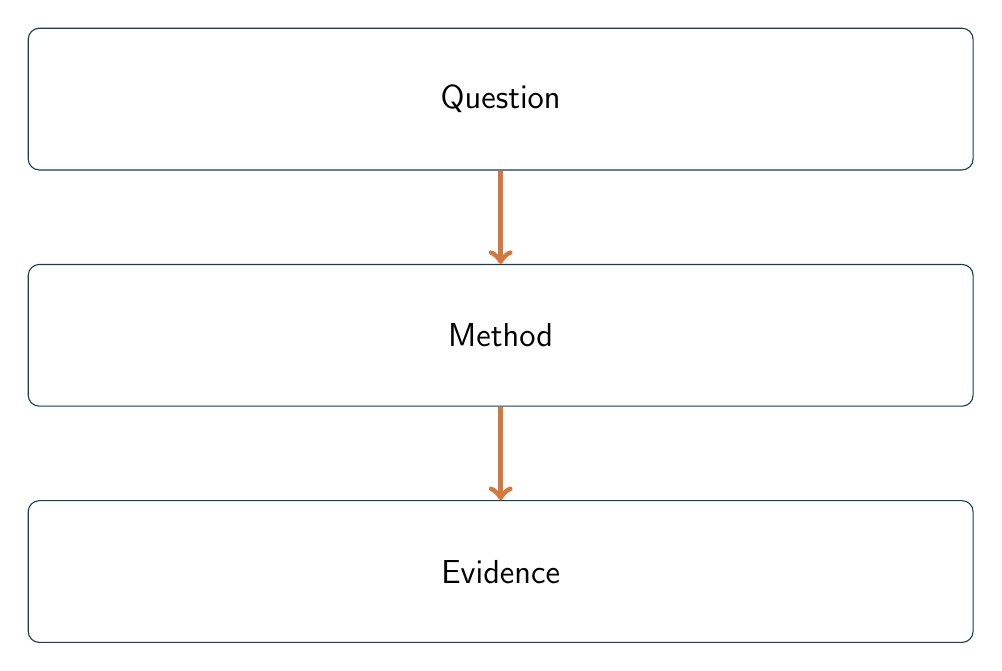
\begin{tikzpicture}[every node/.style={draw=ink,rounded corners,minimum width=12cm,minimum height=18mm,font=\large\sffamily}]
\node (q) at (0,0) {Question};\node (m) at (0,-3) {Method};\node (e) at (0,-6) {Evidence};
\draw[->,line width=2pt,accent] (q)--(m);\draw[->,line width=2pt,accent] (m)--(e);
\end{tikzpicture}\end{center}
\columnbreak
\section*{04 / Example findings}
\begin{tabular}{lrr}\toprule & Baseline & Prototype\\\midrule Task success & 72\% & 89\%\\Reproduction & 65\% & 94\%\\\bottomrule\end{tabular}
\vspace{10mm}{\sffamily\bfseries\color{ink}\fontsize{52}{58}\selectfont 94\%\par}{\Large Example reproduction success\par}
These fictional figures illustrate the layout. Replace them with your results and include uncertainty.
\section*{05 / What we learned}Readers benefit when tools explain the relationship between a result and the decisions that produced it.
\section*{06 / Next steps}Evaluate the workflow in more research settings and publish the supporting materials.
\vspace{10mm}{\bfseries Get in touch}\\alex@example.com\\research.example.com
\end{multicols}\end{document}
